% ============================================================
% ENDSEM REPORT — Part 3: Comparative Analysis + Results
% Paste this AFTER Part 2 in your Overleaf document
% ============================================================

% ============ V. COMPARATIVE ANALYSIS ============
\section{Comparative Analysis}
\label{sec:comparative}

Table~\ref{tab:full_comparison} presents a unified comparison across all reviewed methods, spanning both image and video anomaly detection.

\begin{table*}[t]
\centering
\caption{Unified Comparative Analysis of Reviewed Methods}
\label{tab:full_comparison}
\renewcommand{\arraystretch}{1.3}
\small
\begin{tabular}{@{} l l l c c c c @{}}
\toprule
\textbf{Method} & \textbf{Venue} & \textbf{Domain} & \textbf{Zero-Shot?} & \textbf{Training-Free?} & \textbf{Explainable?} & \textbf{Temporal?} \\
\midrule
PatchCore~\cite{roth2022patchcore} & CVPR '22 & Image & \ding{55} & \ding{55} & \ding{55} & \ding{55} \\
WinCLIP~\cite{jeong2023winclip} & CVPR '23 & Image & \checkmark & \checkmark & \ding{55} & \ding{55} \\
AnomalyCLIP~\cite{zhou2024anomalyclip} & ICLR '24 & Image & \checkmark & \ding{55} & \ding{55} & \ding{55} \\
AnomalyGPT~\cite{gu2024anomalygpt} & AAAI '24 & Image & \ding{55} & \ding{55} & \checkmark & \ding{55} \\
OVVAD~\cite{wu2024ovvad} & CVPR '24 & Video & \checkmark & \ding{55} & \ding{55} & \checkmark \\
LAVAD~\cite{zanella2024lavad} & CVPR '24 & Video & \checkmark & \checkmark & Partial & \checkmark \\
VERA~\cite{ye2025vera} & CVPR '25 & Video & \checkmark & \checkmark & \checkmark & \checkmark \\
\midrule
\textbf{DA-ZVAD (Ours)} & \textit{Proposed} & \textit{Video} & \checkmark & \checkmark & \checkmark & \checkmark \\
\bottomrule
\end{tabular}
\end{table*}

\noindent\textbf{Key Observation:} No single existing framework satisfies all four desiderata---zero-shot, training-free, explainable, and temporally-aware---simultaneously. This gap directly motivates our proposed DA-ZVAD architecture (Section~\ref{sec:proposed}).


% ============ RESEARCH GAP ============
\section{Research Gap}
\label{sec:research_gap}

Our study of the existing literature reveals six recurring shortcomings that cut across both image-based and video-based anomaly detection methods:

\begin{enumerate}[leftmargin=*]
    \item \textbf{Training dependency.} Methods such as PatchCore~\cite{roth2022patchcore}, AnomalyGPT~\cite{gu2024anomalygpt}, and OVVAD~\cite{wu2024ovvad} rely on domain-specific labelled or normal data for each deployment setting. Collecting and annotating such data is expensive and slows down deployment to new environments.

    \item \textbf{Closed-vocabulary detection.} Conventional supervised and weakly-supervised approaches can only flag anomaly categories that were present in the training set. When a previously unseen anomaly type occurs at test time, these models fail without warning.

    \item \textbf{Absence of explainability.} WinCLIP~\cite{jeong2023winclip}, AnomalyCLIP~\cite{zhou2024anomalyclip}, PatchCore, and OVVAD produce numerical anomaly scores or coarse heatmaps, but never state \textit{what} the defect is or \textit{why} it is considered anomalous. In industrial quality control and surveillance, such reasoning is essential for root-cause analysis and regulatory compliance.

    \item \textbf{Domain rigidity.} All reviewed methods assume a fixed deployment environment. However, the definition of ``normal'' is inherently context-dependent---a person running is expected in a sports arena but suspicious in a hospital corridor. None of the existing methods offer a way to adjust the normality baseline across domains without retraining or parameter updates.

    \item \textbf{Lack of temporal reasoning.} CLIP-based methods score each video frame in isolation, treating every frame as a separate image. They cannot capture progressive events---for instance, a person walking, then running, then attacking---where the anomaly only becomes apparent through the temporal sequence.

    \item \textbf{Caption hallucination.} LAVAD~\cite{zanella2024lavad} depends on BLIP-2 captions that can be noisy or factually incorrect. When the LLM reasons over hallucinated captions, the resulting anomaly scores become unreliable, leading to false positives.
\end{enumerate}

These six gaps together point to the need for a method that operates without training data, handles unseen anomaly types, adapts to new domains, models temporal dynamics, and provides human-readable explanations. No existing work satisfies all of these requirements at once.


% ============ PROBLEM STATEMENT ============
\section{Problem Statement}
\label{sec:problem_statement}

The objective of this work is stated as follows:

\begin{quote}
\textit{``Design and Development of a Zero-Shot Video Anomaly Detection System using Vision-Language Models with Domain-Adaptive Verbalized Prompting for Cross-Domain Surveillance and Industrial Monitoring.''}
\end{quote}

\noindent Specifically, the research pursues five objectives:

\begin{enumerate}[leftmargin=*]
    \item Develop a \textbf{training-free} video anomaly detection pipeline built on top of pre-trained Vision-Language Models.
    \item Enable \textbf{domain adaptation} through natural language context descriptions alone, requiring no retraining or parameter changes when the deployment environment changes.
    \item Provide \textbf{natural language explanations} alongside every anomaly score, making detections interpretable for human operators.
    \item Support \textbf{open-vocabulary} detection so that anomaly types never encountered during any training phase can still be identified.
    \item Evaluate the system on \textbf{cross-domain benchmarks}---UCF-Crime, XD-Violence, and MVTec AD---to confirm generalisation across surveillance and industrial settings.
\end{enumerate}


% ============ MATHEMATICAL FORMULATION ============
\section{Mathematical Formulation}
\label{sec:formulation}

Let a video $\mathcal{V}$ consist of $T$ frames:
\begin{equation}
    \mathcal{V} = \{f_1, f_2, \ldots, f_T\}, \quad f_t \in \mathbb{R}^{H \times W \times 3}.
\end{equation}

\noindent The task is to assign each frame an anomaly score. We define a scoring function
\begin{equation}
    \mathcal{S} : \mathbb{R}^{H \times W \times 3} \rightarrow [0, 1],
\end{equation}
where $\mathcal{S}(f_t)$ is close to~1 when frame $f_t$ is anomalous and close to~0 when it is normal. Performance is measured with the frame-level Area Under the ROC Curve:
\begin{equation}
    \text{AUROC} = \int_{0}^{1} \text{TPR}(\tau) \; d\text{FPR}(\tau),
\end{equation}
where $\tau$ is the decision threshold, TPR is the true positive rate, and FPR is the false positive rate.

\medskip
\noindent\textbf{Zero-shot constraint.} Unlike conventional methods that learn from a labelled training set $\mathcal{D}_{\text{train}} = \{(\mathcal{V}_i, y_i)\}_{i=1}^{N}$, our system operates under the constraint
\begin{equation}
    |\mathcal{D}_{\text{train}}| = 0.
\end{equation}
The scoring function relies entirely on a \textit{frozen} VLM $\Phi_{\text{VLM}}$ and natural language prompts $\mathcal{P}$; no model parameters are updated during deployment.

\medskip
\noindent\textbf{Domain-conditioned scoring.} To handle the fact that normality differs across environments, we condition the scoring function on a textual domain context $\mathcal{C}^{t}$ that describes the deployment setting (e.g., \textit{``A warehouse corridor with conveyor belts''}):
\begin{equation}
    \mathcal{S}(f_t \mid \mathcal{C}^{t}) : \mathbb{R}^{H \times W \times 3} \times \mathcal{T} \rightarrow [0, 1],
\end{equation}
where $\mathcal{T}$ is the space of natural language descriptions. Switching to a new domain only requires changing $\mathcal{C}^{t}$; all model parameters remain fixed:
\begin{equation}
    \theta^{s} = \theta^{t} = \theta_{\text{frozen}}.
\end{equation}
This formulation captures the core idea of our approach: domain adaptation through language rather than through parameter updates.

% ============ EVOLUTION DIAGRAM ============
Figure~\ref{fig:evolution} illustrates the evolution of anomaly detection methods from traditional approaches to our proposed framework.

\begin{figure}[h]
\centering
\begin{tikzpicture}[
    node distance=0.5cm,
    block/.style={rectangle, draw, fill=blue!8, text width=5.5cm, minimum height=0.9cm, align=center, rounded corners=3pt, font=\small},
    arrow/.style={-{Stealth[length=2.5mm]}, thick, gray},
    era/.style={font=\footnotesize\bfseries, text=gray}
]

\node[block, fill=orange!15] (trad) {Traditional AD (PatchCore)\\99.1\% AUROC $\mid$ Needs training $\mid$ No explanations};

\node[block, fill=green!12, below=of trad] (clip) {CLIP-based Zero-Shot (WinCLIP, AnomalyCLIP)\\91.8\% AUROC $\mid$ No training $\mid$ No explanations};

\node[block, fill=purple!12, below=of clip] (mllm) {MLLM-based (AnomalyGPT, MMAD)\\94.1\% AUROC $\mid$ Needs fine-tuning $\mid$ Explainable};

\node[block, fill=red!10, below=of mllm] (video) {Video AD (OVVAD, LAVAD, VERA)\\Training-free $\mid$ Temporal $\mid$ Domain-adaptive};

\node[block, fill=yellow!20, below=of video, draw=red!60, line width=1.2pt] (ours) {\textbf{DA-ZVAD (Proposed)}\\Zero-shot + Temporal + Explainable + Domain-adaptive};

\draw[arrow] (trad) -- (clip);
\draw[arrow] (clip) -- (mllm);
\draw[arrow] (mllm) -- (video);
\draw[arrow] (video) -- (ours);

\node[era, left=0.3cm of trad] {2022};
\node[era, left=0.3cm of clip] {2023};
\node[era, left=0.3cm of mllm] {2024};
\node[era, left=0.3cm of video] {2024--25};
\node[era, left=0.3cm of ours] {Proposed};

\end{tikzpicture}
\caption{Evolution of anomaly detection methods. Our proposed DA-ZVAD integrates the strengths of each generation.}
\label{fig:evolution}
\end{figure}


% ============ VI. BASELINE IMPLEMENTATION ============
\section{CLIP Zero-Shot Baseline: Implementation and Results}
\label{sec:baseline}

\subsection{Methodology}

We implement a training-free CLIP-based anomaly detection baseline using OpenCLIP ViT-L/14 (pretrained on LAION-2B). For each MVTec AD category, the model computes image-level anomaly scores via cosine similarity between CLIP image embeddings and an ensemble of normal/abnormal text prompts.

\textbf{Prompt Ensemble Design.} We employ 4 template structures $\times$ 6 state descriptors, yielding 24 prompts per category:

\begin{itemize}[leftmargin=*]
    \item \textbf{Templates:} ``a photo of a \{state\} \{object\}'', ``a \{state\} \{object\}'', ``a \{object\} with \{state\} appearance'', ``a \{state\} looking \{object\}''
    \item \textbf{Normal states:} good, perfect, flawless, normal, pristine, unblemished
    \item \textbf{Abnormal states:} damaged, broken, defective, flawed, abnormal, imperfect
\end{itemize}

The anomaly score is computed as:
\begin{equation}
    s = \frac{\exp(\text{sim}(\mathbf{v}, \mathbf{t}_{\text{abnormal}}) / \tau)}{\exp(\text{sim}(\mathbf{v}, \mathbf{t}_{\text{normal}}) / \tau) + \exp(\text{sim}(\mathbf{v}, \mathbf{t}_{\text{abnormal}}) / \tau)}
\end{equation}
where $\mathbf{v}$ is the image embedding, $\mathbf{t}$ are mean-pooled text embeddings, and $\tau$ is the learned temperature.

\subsection{Results on MVTec AD}

Table~\ref{tab:mvtec_results} presents per-category results on the full MVTec AD test set.

\begin{table}[h]
\centering
\caption{CLIP Zero-Shot Baseline Results on MVTec AD (ViT-L/14)}
\label{tab:mvtec_results}
\renewcommand{\arraystretch}{1.15}
\small
\begin{tabular}{@{} l r r r r @{}}
\toprule
\textbf{Category} & \textbf{Samples} & \textbf{AUROC\%} & \textbf{F1\%} & \textbf{Time (s)} \\
\midrule
\multicolumn{5}{l}{\textit{Textures}} \\
\midrule
Carpet & 117 & \textbf{99.2} & 98.3 & 9.6 \\
Grid & 78 & \textbf{99.7} & 99.1 & 5.3 \\
Leather & 124 & \textbf{100.0} & 100.0 & 8.3 \\
Tile & 117 & 98.7 & 97.6 & 7.9 \\
Wood & 79 & \textbf{100.0} & 100.0 & 6.6 \\
\midrule
\multicolumn{5}{l}{\textit{Objects}} \\
\midrule
Bottle & 83 & 85.6 & 89.5 & 6.1 \\
Cable & 150 & 79.5 & 82.4 & 9.9 \\
Capsule & 132 & 80.9 & 90.8 & 9.3 \\
Hazelnut & 110 & 86.8 & 87.5 & 8.2 \\
Metal Nut & 115 & 84.3 & 90.7 & 7.3 \\
Pill & 167 & 85.6 & 92.0 & 10.1 \\
Screw & 160 & 84.3 & 87.2 & 9.4 \\
Toothbrush & 42 & 90.8 & 91.5 & 6.6 \\
Transistor & 100 & 72.7 & 64.2 & 18.4 \\
Zipper & 151 & 80.3 & 89.5 & 9.2 \\
\midrule
\textbf{Mean (Textures)} & & \textbf{99.5} & \textbf{99.0} & \\
\textbf{Mean (Objects)} & & \textbf{83.1} & \textbf{86.6} & \\
\textbf{Mean (All)} & & \textbf{88.5} & \textbf{90.7} & \\
\bottomrule
\end{tabular}
\end{table}

% ============ AUROC BAR CHART ============
\begin{figure}[h]
\centering
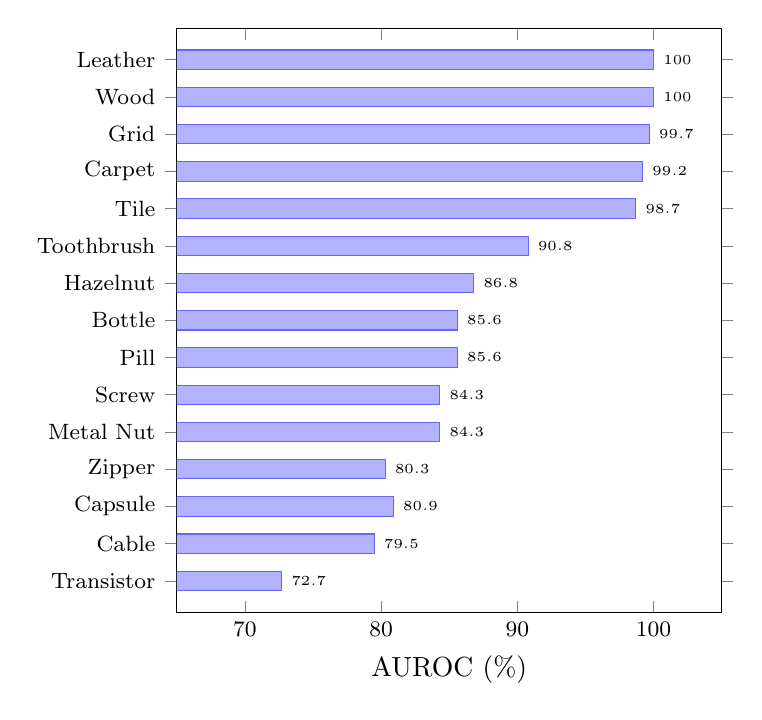
\begin{tikzpicture}
\begin{axis}[
    xbar,
    width=8.5cm,
    height=9cm,
    xlabel={AUROC (\%)},
    xmin=65, xmax=105,
    symbolic y coords={Transistor, Cable, Capsule, Zipper, Metal Nut, Screw, Pill, Bottle, Hazelnut, Toothbrush, Tile, Carpet, Grid, Wood, Leather},
    ytick=data,
    y tick label style={font=\footnotesize},
    x tick label style={font=\footnotesize},
    nodes near coords,
    nodes near coords style={font=\tiny},
    every node near coord/.append style={anchor=west},
    bar width=7pt,
    enlarge y limits={abs=0.4cm},
]
\addplot[fill=blue!30, draw=blue!60] coordinates {
    (72.7,Transistor)
    (79.5,Cable)
    (80.9,Capsule)
    (80.3,Zipper)
    (84.3,Metal Nut)
    (84.3,Screw)
    (85.6,Pill)
    (85.6,Bottle)
    (86.8,Hazelnut)
    (90.8,Toothbrush)
    (98.7,Tile)
    (99.2,Carpet)
    (99.7,Grid)
    (100.0,Wood)
    (100.0,Leather)
};
\end{axis}
\end{tikzpicture}
\caption{Per-category AUROC for CLIP zero-shot baseline on MVTec AD. Textures (top) achieve near-perfect scores; objects show more variation due to subtle, localised defects.}
\label{fig:auroc_bar}
\end{figure}

\subsection{Analysis}

\textbf{Texture vs.\ Object Gap:} Textures achieve a remarkable 99.5\% mean AUROC, while objects achieve 83.1\%. This is expected---texture anomalies (scratches, stains, colour changes) produce global visual differences that CLIP's image-level embeddings capture well, whereas object anomalies (e.g., a bent transistor lead) are highly localised and require spatial reasoning that whole-image CLIP embeddings lack.

\textbf{Comparison with Prior Work:} Our 88.5\% AUROC using simple prompt ensembles approaches WinCLIP's 91.8\% (which uses multi-scale sliding windows for spatial localisation). This 3.3\% gap is attributable to WinCLIP's spatial windowing, which we deliberately omit to maintain a simpler, more extensible baseline suitable for video extension.

\textbf{Inference Speed:} Total evaluation across all 15 categories completes in 135.8 seconds on a single Tesla T4 GPU, demonstrating the practical efficiency of zero-shot approaches.

% ============ VII. VIDEO EXTENSION EXPERIMENT ============
\section{Preliminary Video Extension}
\label{sec:video_experiment}

To demonstrate the extension from image to video anomaly detection, we construct a \textbf{pseudo-video} from MVTec AD bottle images, simulating a quality inspection conveyor belt scenario.

\subsection{Experimental Setup}

We arrange MVTec AD bottle test images as a temporal sequence:
\begin{center}
[Normal $\times$ 10] $\rightarrow$ [Anomalous $\times$ 10] $\rightarrow$ [Normal $\times$ 10]
\end{center}

Each frame is scored independently using CLIP ViT-L/14 with domain-specific prompts (e.g., ``a photo of a good bottle'' vs. ``a photo of a damaged bottle''). This simulates a real-world scenario where a camera monitors products on a conveyor belt and must detect when defective items appear.

\subsection{Results}

\begin{table}[h]
\centering
\caption{Pseudo-Video Frame Scoring Results (MVTec Bottle)}
\label{tab:video_results}
\renewcommand{\arraystretch}{1.2}
\begin{tabular}{@{} l c @{}}
\toprule
\textbf{Metric} & \textbf{Value} \\
\midrule
Mean score (normal frames) & 0.307 \\
Mean score (anomalous frames) & 0.894 \\
Score gap & \textbf{0.587} \\
Total frames & 30 \\
\bottomrule
\end{tabular}
\end{table}

Figure~\ref{fig:temporal_scoring} illustrates the temporal anomaly score profile. The anomaly score clearly spikes when defective frames appear (frames 10--19) and returns to baseline when normal frames resume (frames 20--29), demonstrating CLIP's strong per-frame discriminative ability.

% Temporal score diagram (TikZ approximation)
\begin{figure}[h]
\centering
\begin{tikzpicture}
\begin{axis}[
    width=8.5cm,
    height=5cm,
    xlabel={Frame Index},
    ylabel={Anomaly Score},
    xmin=-1, xmax=30,
    ymin=-0.05, ymax=1.1,
    ytick={0, 0.25, 0.5, 0.75, 1.0},
    xtick={0, 5, 10, 15, 20, 25},
    grid=major,
    grid style={gray!20},
    legend pos=north west,
    legend style={font=\footnotesize},
]

% Normal region shading
\addplot[name path=upper, draw=none, forget plot] coordinates {(-1,1.1) (9.5,1.1)};
\addplot[name path=lower, draw=none, forget plot] coordinates {(-1,-0.05) (9.5,-0.05)};
\addplot[fill=green, fill opacity=0.08, forget plot] fill between[of=upper and lower];

% Anomalous region shading
\addplot[name path=upper2, draw=none, forget plot] coordinates {(9.5,1.1) (19.5,1.1)};
\addplot[name path=lower2, draw=none, forget plot] coordinates {(9.5,-0.05) (19.5,-0.05)};
\addplot[fill=red, fill opacity=0.1, forget plot] fill between[of=upper2 and lower2];

% Normal region 2
\addplot[name path=upper3, draw=none, forget plot] coordinates {(19.5,1.1) (30,1.1)};
\addplot[name path=lower3, draw=none, forget plot] coordinates {(19.5,-0.05) (30,-0.05)};
\addplot[fill=green, fill opacity=0.08, forget plot] fill between[of=upper3 and lower3];

% Threshold line
\addplot[orange, dashed, thick] coordinates {(-1,0.5) (30,0.5)};

% Score line
\addplot[blue, thick, mark=*, mark size=1.5pt] coordinates {
    (0,0.33) (1,0.18) (2,0.27) (3,0.17) (4,0.27)
    (5,0.24) (6,0.30) (7,0.29) (8,0.30) (9,0.35)
    (10,0.60) (11,0.92) (12,0.98) (13,1.0) (14,0.97)
    (15,0.86) (16,0.99) (17,0.97) (18,0.99) (19,0.92)
    (20,0.35) (21,0.15) (22,0.20) (23,0.34) (24,0.44)
    (25,0.43) (26,0.37) (27,0.30) (28,0.29) (29,0.27)
};

\legend{Threshold (0.5), CLIP score}

% Annotations
\node[font=\tiny, text=green!50!black] at (axis cs:4.5,1.03) {Normal};
\node[font=\tiny, text=red!70!black] at (axis cs:14.5,1.03) {Anomalous};
\node[font=\tiny, text=green!50!black] at (axis cs:24.5,1.03) {Normal};

\end{axis}
\end{tikzpicture}
\caption{Temporal anomaly score profile for pseudo-video sequence. CLIP correctly identifies the anomalous segment (frames 10--19) with clear score separation from normal frames.}
\label{fig:temporal_scoring}
\end{figure}

\subsection{Limitations Identified}

While CLIP successfully scores individual frames, the per-frame approach reveals critical limitations that motivate next semester's work:

\begin{enumerate}[leftmargin=*]
    \item \textbf{No temporal context:} Each frame is scored independently---the model cannot detect anomalies that require understanding motion or events over time.
    \item \textbf{Score fluctuations:} Within the anomalous segment, scores fluctuate (0.60--1.0) due to varying defect visibility, with no temporal smoothing.
    \item \textbf{No event reasoning:} The model cannot describe \textit{what happened}---only that a frame looks abnormal.
\end{enumerate}

These limitations directly motivate the integration of temporal adapters (OVVAD), LLM reasoning (LAVAD), and verbalized prompting (VERA) in our proposed architecture.

% END OF PART 3 — Continue with Part 4
